\section{Methodology}
In this section, we provide an overview of how we collected our dataset and the algorithms that we utilize to understand the interactions among Twitter users and with different topics. 

\subsection{Estimating Partisanship\label{sec:background-ca}}

To approximate individual Twitter users' partisanship, we rely on the Correspondence Analysis (CA) proposed by Barber{\'a} {et~al.}~\cite{barbera2015tweeting}.  Correspondence analysis (CA), similar to principal component analysis, is a technique for categorical data that extracts discriminating and representative features from a given matrix~\cite{greenacre2010correspondence}. As found by Barber{\'a} {et~al.}, individual users often reveal their political preferences by whom they choose to follow on Twitter, and by analyzing these choices using CA, we can approximate their place on the political-ideological spectrum. CA works as follows: Given an $n \times m$ adjacency matrix that indicates whether user $i$ (row) follows user $j$ (column), CA can determine a discriminating latent space among these users based on their following behaviors. By carefully choosing our set of ``followed'' users (columns of the matrix) as a set of key political figures, this latent space can be used to represent a dimension of ``partisanship.'' Then, considering individuals' place on the left/right US political spectrum as a point within this latent space, we can estimate that point by projecting them onto the latent space based on who they choose to follow.\footnote{We utilize the Tweepy API to identify the set of users that each of our non-target political accounts follows.} The result is that if a given user follows many liberal-leaning/democratic or a set of accounts that liberal-leaning accounts tend to follow, then we consider that account to be liberal, and vice versa~\cite{barbera2015tweeting,mcpherson2001birds}. We note that with the CA technique, by later extending the set of the key followed accounts, this approach can be used to approximate the partisanship of users who do not necessarily follow one of the initial set of key political figures (\textit{e.g.}, congressional leaders).

\begin{figure}
\begin{minipage}[l]{0.47\textwidth}
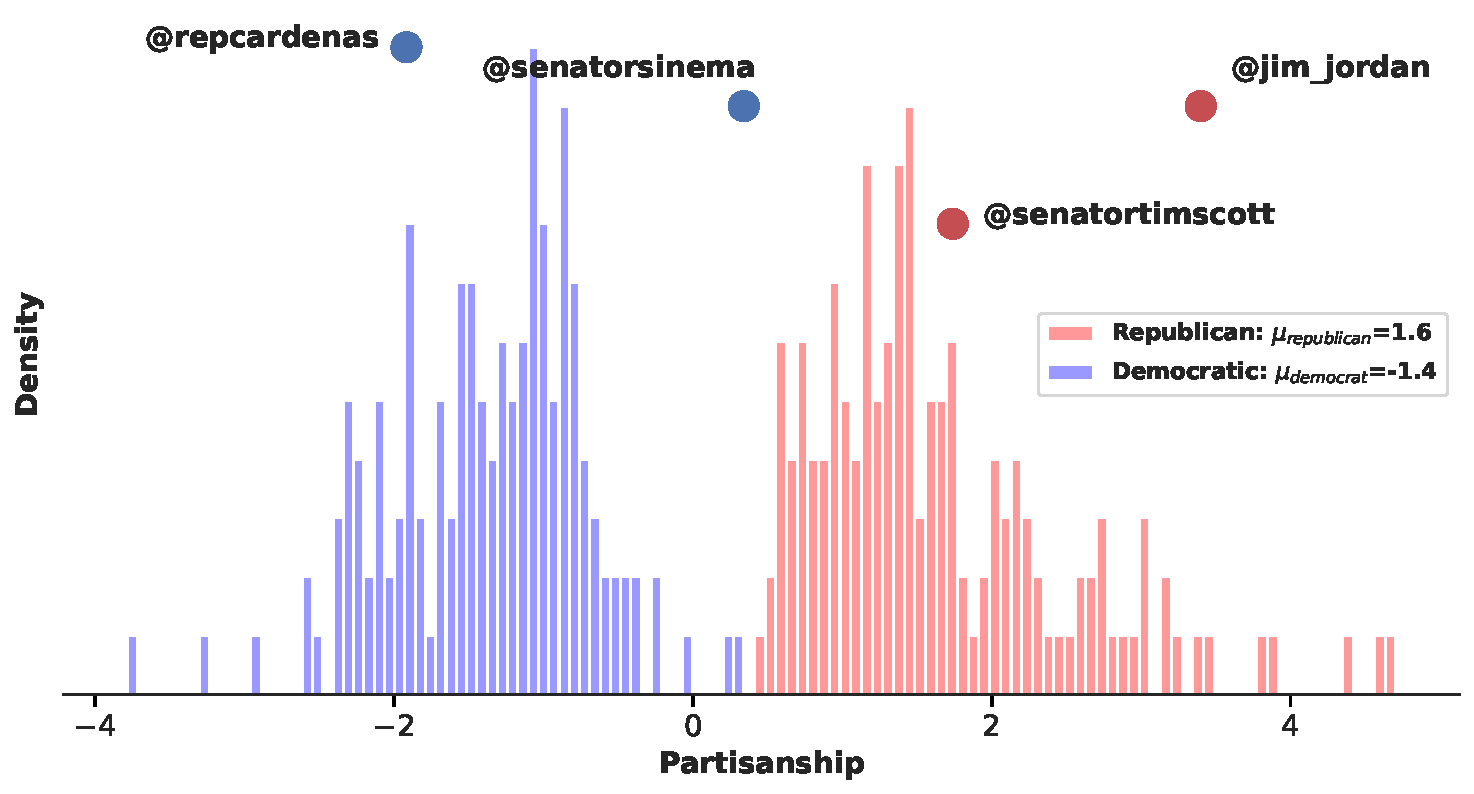
\includegraphics[width=1\columnwidth]{figures/partisanship_us_members-20240424.pdf} 
\end{minipage}
\begin{minipage}[l]{0.47\textwidth}
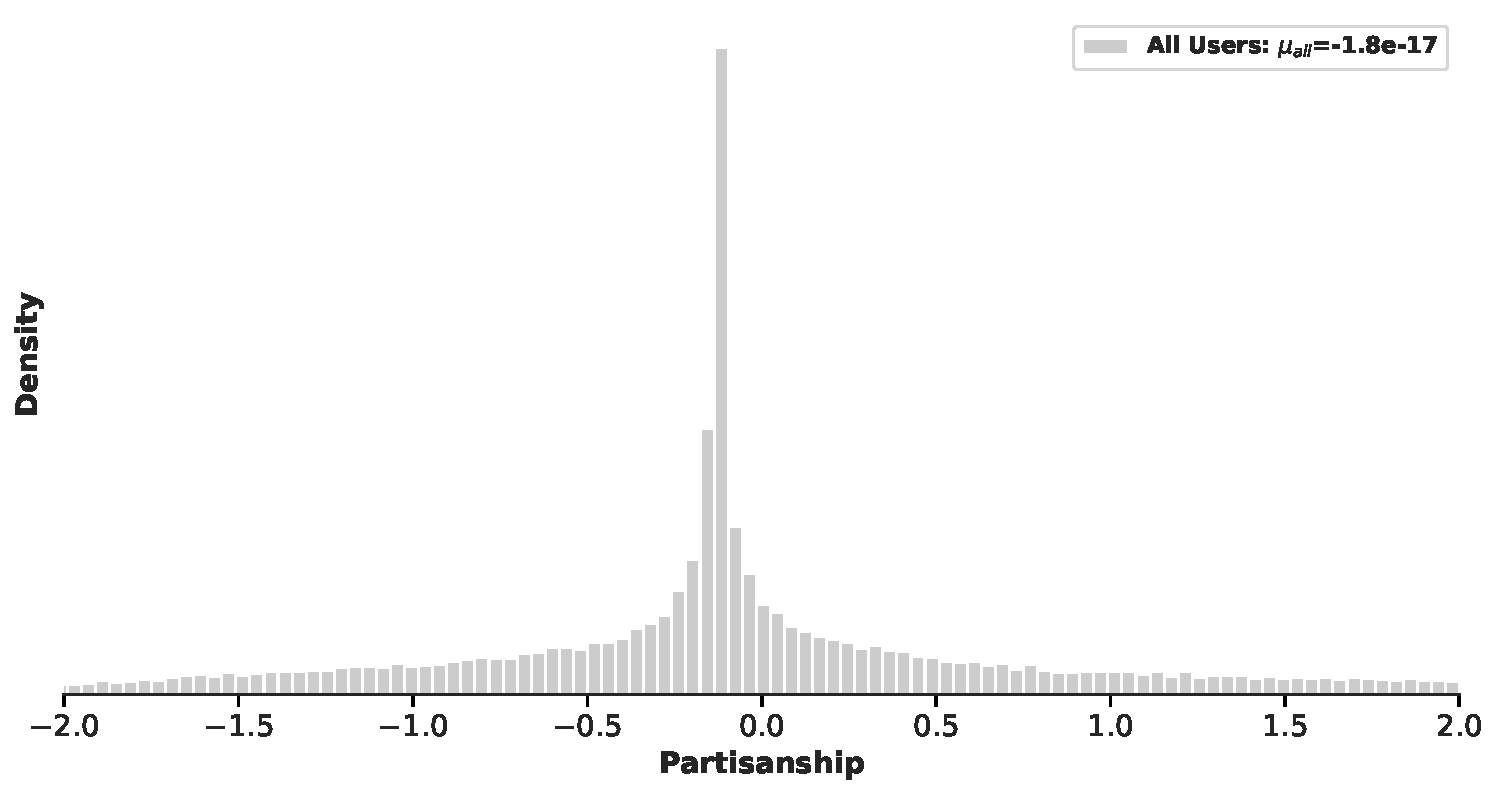
\includegraphics[width=1\columnwidth]{figures/partisanship_all_users-20240424.pdf} 
\end{minipage}

\begin{minipage}[l]{1\textwidth}
\caption{{Estimated Political Orientation of Political Leaders and All Users Using CA}-- We differentiate users' political leanings based on who they follow on Twitter.\label{fig:politican-orientation}}
\end{minipage}

\end{figure}
We note that for our initial set of key political predictive ``followed'' accounts,  we utilize the Twitter accounts of the US House of Representatives and US Senate members from the 117th Congress (2021--2023). In addition to these accounts, we further add another 352~political accounts that were formerly identified by Barber{\'a} {et~al.} (\textit{e.g.,} $@$JoeBiden, $@$VP).\footnote{\url{https://github.com/pablobarbera/twitter_ideology}} Using these accounts, and following the approach as specified by  Barber{\'a}  {et~al.}, we subsequently identified a politically ideological subspace and projected our final list of 43,151 different accounts to this subspace. See Appendix~\ref{sec:appendix-ca} for 
 additional details. As seen in Figure~\ref{fig:politican-orientation}, using this method we manage to obtain a discriminating latent space that allows us to differentiate the ideology of Republican and Democratic political leaders as well as our set of 43,151 accounts. In this setup, the more positive a user's ideology, the more right-leaning; the more negative, the more left-leaning.  

\subsection{Collecting Tweets}
Our dataset initially consisted of 187.6M tweets from 55.4K users that followed our set of key political figures. We collected this data utilizing the Twitter API throughout 2022. We note that following the acquisition of Twitter by Elon Musk, access to the API became restricted limiting our analysis to this time period~\cite{Singh2023}.  Upon identifying these users, given that our work is primarily focused on the US political system, we removed any user that listed their location on their Twitter profile as outside of the United States. To identify US-based users, we utilize the capability of the \texttt{Nominatim} Python tool to geo-code all user's locations based on their Twitter-provided location string and OpenStreetMap.\footnote{\url{https://www.openstreetmap.org/}} Altogether, we remove 12,264 users, leaving us 43,151 users. Upon identifying our user subset, we subsequently utilize \texttt{whatlango}\footnote{\url{https://github.com/abadojack/whatlanggo}} Go library to remove any non-English tweets from our set of users, leaving us 89,599,787 tweets. While we acknowledge several of our users' tweets might have been deleted or taken down by Twitter administrators before we scraped them, this dataset, consisting of over 89.6 million tweets, with an average of 2076.4 (median 614.0) tweets per individual is largely comprehensive of each user's tweeting behavior on the platform.




\subsection{Determining the Toxicity of Tweets\label{sec:labeling-toxic}}

%\subsubsection{Designing an Open-Source Toxicity Classifier}
We design and open-source\footnote{The weights for our model can be downloaded at \url{https://www.github.com/REDACTED}} a contrastive DeBERTa-based~\cite{he2022debertav3} model to determine the toxicity of tweets, later benchmarking our approach on two public datasets and against the Perspective Toxicity API~\cite{perspectiveapi}, the gold standard of toxicity detection~\cite{perspectiveapi,kumar2021designing,rajadesingan2020quick}. We note that throughout our work, we reproduce several results using the Perspective Toxicity classifier and present them in the appendix after obtaining similar results.
To train our new model we rely on the Civil Comments dataset\footnote{\url{https://www.kaggle.com/competitions/jigsaw-unintended-bias-in-toxicity-classification/data}} that was also utilized to train and validate the Perspective API. In addition to utilizing this dataset to augment our trained model, we take two main approaches: (1) data augmentation through realistic adversarial perturbations of the original Civil Comments dataset~\cite{le2022perturbations}, and (2) the inclusion of a contrastive learning embedding layer to help better differentiate toxic and non-toxic texts. For training details of our new model, see Appendix~\ref{sec:app-tox-classifier}.


\vspace{2pt}\noindent
\noindent
\textbf{Benchmarking our Toxicity Classifier.}
Upon training our toxicity model, we compare its performance against the Perspective Toxicity API~\cite{perspectiveapi} and a vanilla finetuned DeBERTa model with a classification head (a two-layer MLP with ReLU activation). To benchmark our toxicity model, we utilize the validation and test dataset of the Civil Comments dataset provided by Google Jigsaw\cite{perspectiveapi} as well as a separate toxicity dataset provided by Kumar {et~al.}~\cite{kumar2021designing}. Kumar  {et~al.}'s datasets consist of 107,620~social media comments (including from Twitter) where each comment was labeled by 5 human annotators as toxic or not (as opposed to the 10 annotators in the Civil Comments dataset). For our $F_1$ score calculations, as in Kumar {et~al.}~\cite{kumar2021designing} and in the Civil Comments dataset, we consider a comment to be toxic if its toxicity $t_i > 0.5$. Again, we utilize this threshold for classifying a comment as toxic, given that this score (as described in the Civil Comments task) indicates that a majority of the Civil Comments annotators would have assigned a ``toxic'' attribute to this comment.

As seen in Table~\ref{tab:benchmark-toxicity}, our contrastive DeBERTa model achieves the lowest mean absolute error (MAE) as well as the highest Pearson correlation and $F_1$ scores across the Civil Comments validation and test dataset. In addition, while obtaining a slightly lower correlation, our model on this separate dataset achieves a lower mean absolute error and a higher $F_1$ score. As such for the rest of this work, when determining the toxicity of tweets, we utilize our contrastive DeBERTa model. We note that our model has a $\rho= 0.870$ Pearson correlation with the scores output by the Perspective API, illustrating its use as an offline alternative with competitive performance to Perspective. Lastly, for this work, as in other works~\cite{hanley2023sub, rajadesingan2020quick}, when determining the overall toxicity of users, or particular groupings of tweets, we utilize the average of the toxicity scores of the tweets output by our model. 
 

\begin{table*}
\centering
\fontsize{8.4pt}{6}
\selectfont
\begin{tabular}{l|ccc|ccc|ccc}
\toprule
& \multicolumn{3}{c|}{\textbf{CC Validation}} & \multicolumn{3}{c|}{\textbf{CC Test }} & \multicolumn{3}{c}{\textbf{Kumar {et~al.} }} \\

Model & MAE & Corr. &Macro-$F_1$ & MAE & Corr. &Macro-$F_1$&  MAE & Corr. &Macro-$F_1$\\ \midrule
DeBERTa & 0.0650 &0.800 &0.841 & 0.0654& 0.797 &0.842 & \textbf{0.241} & 0.383 & 0.539  \\
DeBERTa-contrastive & \textbf{0.0601} &\textbf{0.820} &\textbf{0.851} & \textbf{0.0609}& \textbf{0.818}&\textbf{0.852} & {0.251} & 0.415 & \textbf{0.540}  \\
Perspective API & 0.0961& 0.778& 0.845& 0.0963& 0.777 & 0.842 & 0.332 & \textbf{0.417} & 0.410 \\
\bottomrule
\end{tabular}
\vspace{3pt}
\caption{\label{tab:benchmark-toxicity} Mean absolute error, Pearson correlation, and $F_1$ score of the Perspective API and our DeBERTa models on the Civil Comments Validation and Test dataset. We bold the best scores in each respective column  }
\vspace{-10pt}
\end{table*}




 
\subsection{Topic Analysis with MPNet and DPMeans\label{sec:topic-background}} To later understand how particular types of users interact with different topics composed of toxic tweets, we perform topic analysis on these messages. As found by Grootendorst {et~al.}~\cite{grootendorst2020bertopic,hanley2023partial}, by embedding small messages like Tweets into a shared embedding space and then clustering these embeddings, fine-grained and highly specific topics can be extracted from datasets. To do this, we utilize the large language model MPNet\footnote{\url{https://huggingface.co/sentence-transformers/all-mpnet-base-v2}} fine-tuned on semantic search and a parallelizable minibatch version of the DP-Means algorithm.\footnote{\url{https://github.com/BGU-CS-VIL/pdc-dp-means}}

\vspace{2pt}\noindent
\noindent
\textbf{Fine-tuning MPNet for Topic Analysis.} To compare two tweets' semantic content for later clustering, we rely on a version of the MPNet~\cite{song2020mpnet} large language model that was fine-tuned on semantic search. MPNet maps sentences and paragraphs to a 768-dimensional space, comparing different sentence and paragraph embeddings' semantic content based on cosine similarities (ranging from -1 [highly different] to +1 [highly similar]). We note that the version of MPNet that we utilize was initially fine-tuned on similar social media data (\textit{e.g.}, Reddit comments, and Quora Answers) allowing us to apply this model to our set of tweets. However, to further ensure that our MPNet model is properly suited to our Twitter dataset, as in Hanley et al.~\cite{hhanleyspecious2024}, we further fine-tune this model using an unsupervised contrastive learning objective(\textit{i.e.}, the SimCSE training objective) to better the quality of our embeddings~\cite{gao-etal-2021-simcse}  on our set of tweets. As training data for this fine-tuning, we utilize 1 million tweets randomly sampled from our set of 89.6 million tweets.  See Appendix~\ref{sec:finetune} for additional details. As a reference, we provide two example tweet pairs with similarities at 0.55 and -0.18 in Figure~\ref{figure:paragraph_pairs}. We note that for each tweet within our dataset, before embedding the message, we first remove all URLs, ``@'', ``\#'', emojis, photos, and other non-textual elements from the message. In addition, for each user handle or text hashtag that utilizes camel case (\textit{i.e.}, camelCase) or snake case (\textit{i.e.}, snake\_case), we finally unroll those strings to their constituent elements.


\begin{figure}




\begin{minipage}{1\textwidth}
\hspace{100pt}
\tiny
\textbf{0.735 similarity}
\hspace{120pt}
\tiny
\textbf{-0.032 similarity}
\end{minipage}





\noindent\fcolorbox{black}{lightgray}{%
\begin{minipage}{.44\textwidth}
\tiny
\textbf{Tweet 1:} AZ voters; we need your vote for 
@Adrian\_Fontes and the rest of the Blue ticket. Please, for us, for our children. Please.
\textbf{Tweet 2:} Please vote for 
@Adrian\_Fontes
 and save AZ
\end{minipage}}
\noindent\fcolorbox{black}{lightgray}{%
\begin{minipage}{.44\textwidth}
\tiny
\textbf{Tweet 1:}If a supervisor was giving off those kinds of vibes to a worker in a conventional workplace, an HR complaint would definitely be warranted. Creepy AF


\textbf{Tweet 2:} The close relationship between politics and economics is neither neutral nor coincidental. Large governments evolve through history in order to protect large accumulations of property and wealth.”
\end{minipage}}
\caption{Examples of  Tweet pairs at different similarities (0.735 left and -0.032 right).  }


\label{figure:paragraph_pairs}
\vspace{-10pt}
\end{figure}



\vspace{2pt}\noindent
\noindent
\textbf{DPMeans for Clustering Tweets.}
DP-Means~\cite{dinari2022revisiting} is a non-parametric extension of the K-means clustering algorithm. When running DP-Means, when a given datapoint is a chosen parameter $\lambda$ away from the closest cluster, a new cluster is formed, and that datapoint is assigned to it. This characteristic of DP-Mans enables us to specify how similar individual items must be to one another to be part of the same cluster. Similarly, because DP-Means is non-parametric in terms of the number of clusters formed, we do not need to know \textit{a priori} how many topics are present within our dataset. For additional details about DP-Means, see Appendix~\ref{sec:ap-dpmeans}.

\begin{figure}

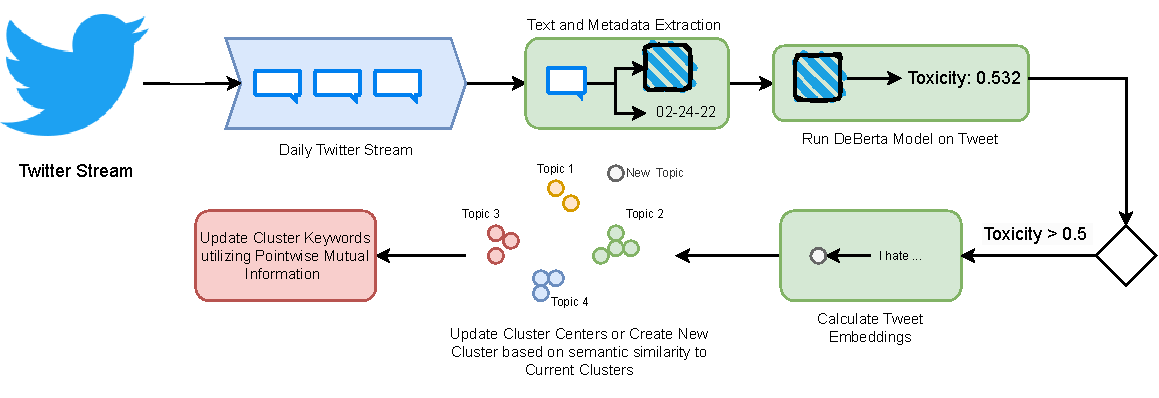
\includegraphics[width=0.9\columnwidth]{figures/Toxic-clustering_documents.drawio.pdf} 
 \caption{Topic analysis of Toxic Tweets---We determine the toxicity, embed, and cluster toxic tweets to identify the most polarized and toxic conversations on Twitter throughout 2022. We note that for this approach, we limit our analysis to English tweets. We utilize the \texttt{whatlango} Go library to determine the language of tweets. \label{fig:toxic-cluster}}
\end{figure}


\vspace{2pt}\noindent
\noindent
\textbf{Topic Analysis Pipeline.}
Having outlined the constituent elements of our topic analysis algorithm, we now go over the full topic analysis pipeline (Figure~\ref{fig:toxic-cluster}): Throughout 2022, as we gathered the tweets of our set of 43,151 Twitter users, using our DeBERTa-contrastive model, we identify potentially toxic tweets (\textit{i.e.}, toxicity $t_i$ > 0.50). Following the identification of these potentially toxic tweets and separating out non-English tweets with \texttt{whatlango}, using MPNet, we subsequently map these tweets to a shared embedding space. Finally, we continuously cluster these tweets to identify topics amongst these toxic tweets using the DP-Means algorithm. To make these clusters that represent topics amongst our set of tweets, human-understand we employ two different approaches. First, we designate the tweets closest (\textit{i.e.}, with the largest cosine similarity) to the center of the cluster as the ``representative tweet'' of the cluster~\cite{grootendorst2020bertopic}. Second, we determine the most distinctive keywords of each cluster using pointwise mutual information~\cite{bouma2009normalized} (detailed in Appendix~\ref{sec:pmi}). In this way, after clustering our set of tweets, we can later extract the semantic meaning of the various clusters outputted. 

As recommended by Hanley {et~al.} we utilize a $\lambda$ of 0.60 for our clusters (precision near 0.989 for MPNet~\cite{hanley2022happenstance,grootendorst2020bertopic}). Finally, we extract keywords from these clusters using the pointwise mutual information metric and determine the most representative tweets by determining the tweet with the highest cosine similarity to the cluster center. Altogether, across the 5,509,042~English-language toxic tweets from our set of 43,151~Twitter users, we identified 5,288~clusters with at least 50~toxic tweets. 

\subsection{Generalized Additive Models}
Throughout this work, we utilize Generalized Additive Models (GAM)~\cite{hastie2017generalized} to determine the relationships between our variables of interest (\textit{e.g.}, user partisanship, and user toxicity). For GAMs, the relationship between the independent and dependent variables is not assumed to be linear but is rather estimated as a smooth regularized nonparametric function. Namely, given a dependent variable $Y$ and a set of $p$ independent variables  $X$, GAM's are estimated as:
\begin{equation}
    g(E(Y))=\alpha+s_1(x_1)+\cdots+s_p(x_p),
\end{equation} where $g()$ is a linking function that connects the expected value of the dependent variable $Y$ to values of functions $s_i()$ of independent independent variables in $X$. For example, when estimating probabilities the logit function is often utilized as with ordinary Generalized Linear Models~\cite{demaris1992logit}. The functions $s_i()$ represent smooth nonparametric functions of the variables in $X$ that are fully determined by the data in $X$ rather than by a parametric function. For GAMs, these $s_i()$ are estimated simultaneously, and the estimated value of $g(E(Y))$ is determined by implying adding up the values of the $s_i()$ functions. Throughout this work, we utilize the Python \texttt{Pygam} library to fit our regressions and utilize the Generalized Cross Validation Loss Criteria (GCV)~\cite{demaris1992logit} for estimating the $s_i()$ functions when fitting. The Generalized Cross-Validation Loss Criteria takes a LOOCV (Leave One Out Cross-Validation) approach to fitting smoothers on the data in X. 

Utilizing GAMS versus other more traditional models allows us  (1) to not assume linear relationships between our dependent and independent variables, and (2) to have better interpretability given that the partial contribution of a given variable $x_i$ to determining the value of the dependent variable Y is a function only of its corresponding function $s_i()$. 

\subsection{Ethical Considerations} 
Within this work, we largely focus on identifying large-scale trends in how different Twitter interact with one another. While we do calculate toxicity and polarization levels for individual users, we only display the names of verified public users or users with more than 500K followers, redacting the names of all other accounts. 
We lastly note that our Twitter data was largely collected before Elon Musk's private acquisition of Twitter on October 27, 2022, and all of our data was collected before the later restrictions placed on the collection of tweets on June 30, 2023.\footnote{\url{https://help.twitter.com/en/rules-and-policies/twitter-limits}}


